
\documentclass{article}
\usepackage{amsmath}
\usepackage{xcolor}
\usepackage{amsthm}
\usepackage{graphicx}
\usepackage{hyperref}
\usepackage{datetime}
\usepackage{outlines}

\newdateformat{monthyeardate}{\monthname[\THEMONTH] \THEYEAR}

\newcommand{\newmarkedtheorem}[1]{%
  \newenvironment{#1}
    {\pushQED{\qed}\csname inner@#1\endcsname}
    {\popQED\csname endinner@#1\endcsname}%
  \newtheorem{inner@#1}%
}

\theoremstyle{definition}
%\newtheorem{eg}{Example}[section]
\newmarkedtheorem{eg}{Example}[section]
\newtheorem{observation}{Observation}[section]
\newtheorem{define}{Definition}[section]
\theoremstyle{plain}
\newtheorem{proposition}{Proposition}[section]
\newtheorem{theorem}{Theorem}[section]
\newtheorem{assump}{Assumption}[section]
\newtheorem{remark}{Remark}[section]

\title{Regeneration Vehicle Partitioning}
\author{Jeroen van Riel}
\date{\monthyeardate\today}

\begin{document}

\maketitle

\section{Conjecture}

Let us first provide some words on notation. We use $t_{j}^{0}$ to denote the
arrival time of some vehicle $j$. The \textit{switch-over} time between vehicles
crossing from different lanes is denoted by $s$. We use $\phi_{W}$ to denote
\textit{partial schedule} on the vehicles $W$, which is a mapping
$\phi: W \rightarrow [0, \infty)$. We write $\sigma_{W}$ whenever this schedule
is (part of) and optimal schedule.

\begin{define}[Regeneration Vehicle]
  Let $V$ be a set of vehicles and $\phi_{V}$ some partial schedule. Vehicle $j^{*}$
  is a regeneration vehicle for $\phi_{V}$ whenever
  \begin{align}
    \phi_{V}(l) \leq t_{j^{*}}^{0} - s
  \end{align}
  for all $l \in V$ with $t_{l}^{0} \leq t_{j^{*}}^{0}$.
\end{define}

Stated in the notation used here, the conjecture from
\cite{limpensOnlinePlatoonForming2023} can be formulated as follows.

\begin{proposition}[Regeneration Vehicle Partitioning]
  Let $V$ be a set of vehicles. Let $W \subset V$ be a subset containing the $k$ earliest arriving vehicles. Suppose that an optimal schedule $\sigma_{W}$ contains a regeneration vehicle $j^{*}$, then we have
  \begin{align}
    \sigma_{V}(l) = \sigma_{W}(l) ,
   \end{align}
   for all vehicles $l \in A = \{ l \in W : t_{l}^{0} < t_{j^{*}}^{0} \}$ that
   arrived before $j^{*}$.
\end{proposition}

\section{Counterexample}

Let $r = r_{2} - r_{1}$ and consider the schedule in the next figure.
\begin{figure}[h]
  \centering
  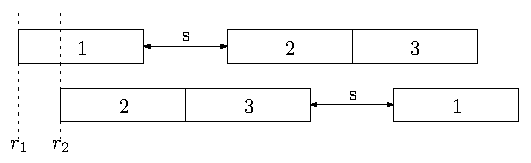
\includegraphics[width=0.5\textwidth]{figures/123.pdf}
\end{figure}
The first schedule has $\sum C_{j} = 6p + 2s$ and the second schedule has
$\sum C_{j} = 3r + 6p + s$. Therefore, the second schedule is optimal whenever
\begin{align}
  \label{eq:counter-assump1}
  r < s / 3 .
\end{align}

Now consider the situation in which we have an additional job $4$ with release
date $r_{4} = 6p + 2s$. It is never optimal to schedule $4$ before any of the
other jobs, so the figure shows the two schedules to consider.
The first schedule has $\sum C_{j} = 10p + 4s$ and the second schedule has
$\sum C_{j} = 10p + 3s + 4r$. Therefore, the first schedule is better assuming
\begin{align}
  \label{eq:counter-assump2}
  r > s/4 .
\end{align}
For $W = \{1, 2, 3, 4\}$, let this schedule be denoted by $\sigma_{W}$.
Observe that vehicle 4 is a regeneration vehicle for $\sigma_{W}$.

\begin{figure}[h]
  \centering
  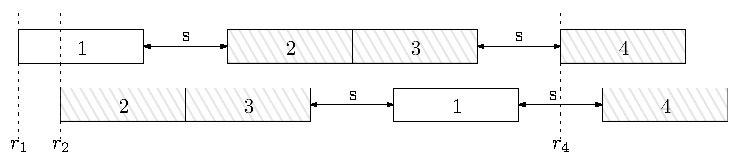
\includegraphics[width=0.72\textwidth]{figures/1234.pdf}
\end{figure}

Now assume that \eqref{eq:counter-assump1} and \eqref{eq:counter-assump2} hold.
Consider two additional jobs 5 and 6 with release date
$r_{5} = r_{6} = r_{4} + r$. Again, we see that vehicles 4, 5 and 6 should be
ordered as $5,6,4$, so it is not hard to reason that the optimal schedule is
given in the figure below and has $\sum C_{j} = 21p + 8s + 6r$. For
$V = \{ 1, \dots, 6\}$, this shows that $\sigma_{V}(l) \neq \sigma_{W}(l)$ for
$A=\{1, 2, 3 \}$.

\begin{figure}[h]
  \centering
  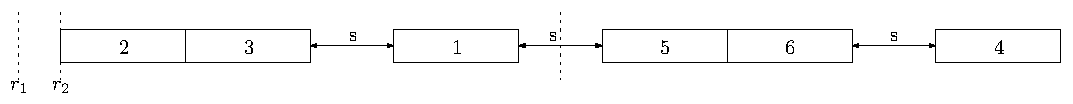
\includegraphics[width=1.0\textwidth]{figures/12345.pdf}
\end{figure}


\bibliography{references}
\bibliographystyle{ieeetr}


\end{document}
